
%(BEGIN_QUESTION)
% Copyright 2007, Tony R. Kuphaldt, released under the Creative Commons Attribution License (v 1.0)
% This means you may do almost anything with this work of mine, so long as you give me proper credit

Determine how each control action (P, I, and D) would react during the periods marked on this process trend by using the symbols $\uparrow$ (driving up), $\downarrow$ (driving down), $+$ (positive), $-$ (negative) or 0 (zero), compared to the actions of each at the beginning of the trend.  Do this for P, as well as for I and D.  Assume {\it direct action} for the controller.

$$\includegraphics[width=15.5cm]{i01641x01.eps}$$

\underbar{file i01641}
%(END_QUESTION)





%(BEGIN_ANSWER)

$$\includegraphics[width=15.5cm]{i01641x02.eps}$$

%(END_ANSWER)





%(BEGIN_NOTES)


{\bf Period 1:}
 

\begin{itemize}
\item{}P is decreasing, because error is becoming more negative
\item{}I is decreasing, because error is negative
\item{}D is negative, because rate of error change is negative
\end{itemize} 
\bigskip 
 

{\bf Period 2:}
 

\begin{itemize}
\item{}P is increasing, because error is becoming more positive
\item{}I is decreasing, because error is negative
\item{}D is positive, because rate of error change is positive
\end{itemize} 
\bigskip 
 

{\bf Period 3:}
 

\begin{itemize}
\item{}P is increasing, because error is becoming more positive
\item{}I is increasing, because error is positive
\item{}D is positive, because rate of error change is positive
\end{itemize} 
\bigskip 
 

{\bf Period 4:}
 

\begin{itemize}
\item{}P is decreasing, because error is becoming more negative
\item{}I is increasing, because error is positive
\item{}D is negative, because rate of error change is negative
\end{itemize} 
\bigskip 
 

{\bf Period 5:}
 

\begin{itemize}
\item{}P is decreasing, because error is becoming more negative
\item{}I is decreasing, because error is negative
\item{}D is negative, because rate of error change is negative
\end{itemize} 
\bigskip 
 

{\bf Period 6:}
 

\begin{itemize}
\item{}P is negative, because error is steady and negative
\item{}I is decreasing, because error is negative
\item{}D is zero, because error is unchanging
\end{itemize} 



%INDEX% Control, proportional + integral + derivative: relative directions of action

%(END_NOTES)


